% main.tex — entry point for the CIT (LNTU) submission.
% Toolchain: pdflatex -> bibtex -> pdflatex -> pdflatex.
% Build:     latexmk -pdf main.tex
%
% See README.md for journal formatting checklist and required section order.

\documentclass[11pt,a4paper,twoside]{article}

% ---- Encoding & languages. T2A for Cyrillic, T1 for Latin.
\usepackage[T2A,T1]{fontenc}
\usepackage[utf8]{inputenc}
\usepackage[english,ukrainian]{babel}
% English is set as the *last* loaded language in babel options so it becomes
% the document's main language; switch to Ukrainian inline via
% \foreignlanguage{ukrainian}{...} or \selectlanguage{ukrainian}.
\selectlanguage{english}

% ---- Times-equivalent for pdfLaTeX.
\usepackage{newtxtext}
\usepackage{newtxmath}

% ---- Quotes: Ukrainian angle quotes « ».
\usepackage{csquotes}

% ---- Hyperlinks (kept quiet — no coloured boxes).
\usepackage[hidelinks]{hyperref}
% expansion disabled because the Cyrillic LH bitmap fallback isn't scalable.
\usepackage[protrusion=true,expansion=false]{microtype}

% ---- Tables (MCP tool surface) and code listings (C# excerpts).
\usepackage{array}
\usepackage{tabularx}
\usepackage{listings}

% Numerical citation marks like [1], [3].
\usepackage[numbers,square,sort&compress]{natbib}

% ---- Project-local style.
\usepackage{cit-style}

\begin{document}

% Header: UDC, ORCID, authors, affiliations, title.
% sections/header.tex — UDC, DOI, authors, ORCID, affiliations, title.
% Layout per the journal's ZRAZOK example: left-aligned author block at 11 pt,
% title centred and bold below the affiliation block.

\noindent
\textbf{DOI:}~\textit{(assigned by editor)}\\
\textbf{УДК}~\textit{$\langle$placeholder — to confirm$\rangle$}\\[0.4em]
\textbf{Богусевич Олексій Олександрович}\textsuperscript{1},
  \textit{$\langle$degree/title$\rangle$}\\
\href{https://orcid.org/0000-0000-0000-0000}{https://orcid.org/0000-0000-0000-0000}\\
\textbf{Свистунов Антон Олександрович}\textsuperscript{1},
  \textit{$\langle$degree/title$\rangle$}\\
\href{https://orcid.org/0000-0000-0000-0000}{https://orcid.org/0000-0000-0000-0000}\\
\textsuperscript{1}\foreignlanguage{ukrainian}{Київський національний університет імені Тараса Шевченка, факультет комп'ютерних наук та кібернетики, м. Київ, Україна}\\

\begin{center}
{\fontsize{14}{16}\selectfont\textbf{PARCS-Agent: An MCP-Mediated Bridge from LLM Agents to Distributed Compute Clusters}}
\end{center}


% Bilingual abstracts + keywords.
% sections/abstract-en.tex --- English abstract + keywords (9 pt, 1 cm indent).

\begin{citabstract}
\noindent\textbf{Bohusevych O., Svystunov A. PARCS-Agent: An MCP-Mediated Bridge from LLM Agents to Distributed Compute Clusters.}
Contemporary large language model (LLM) agents invoke external tools for information retrieval, code execution, and application-programming-interface access; each such invocation runs, however, as a local synchronous function inside a single process. Compute-bound subtasks (Monte Carlo simulation, hyperparameter exploration, combinatorial search) are therefore constrained to the agent's single execution thread, and no standardised mechanism exists for an agent to acquire additional computational resources during task execution. This paper proposes PARCS-Agent, an architectural pattern in which a server implementing the Model Context Protocol (MCP) provides an interface to a Kubernetes-based PARCS distributed computing cluster and exposes a compact set of tools enabling the agent to submit arbitrary C\# computation logic at runtime. The platform compiles the submitted source using Roslyn, distributes execution across daemon worker pods through Kubernetes Event-Driven Autoscaling (KEDA), and propagates intermediate results between successive parallel layers. The agent generates only per-worker logic in straight-line code, thereby circumventing the documented limitations of LLMs in producing correct MPI, OpenMP, and CUDA programs. Bulk input data is delivered through a content-addressed shared-storage side channel, decoupling dataset volume from protocol payload. The approach is illustrated by a Monte Carlo Value-at-Risk case study; quantitative evaluation is reserved for a subsequent publication.

\medskip
\noindent\textbf{Keywords:} AI agents; large language models; Model Context Protocol;
distributed computing; parallel computation; LLM tool use; Kubernetes;
agent infrastructure.
\end{citabstract}

% sections/abstract-uk.tex --- Ukrainian abstract + keywords (9 pt, 1 cm indent).

\begin{otherlanguage}{ukrainian}
\begin{citabstract}
\noindent\textbf{Богусевич О.~О., Свистунов А.~О. PARCS-Agent: міст від агентів великих мовних моделей до розподілених обчислювальних кластерів через протокол MCP.}
Сучасні агенти на основі великих мовних моделей використовують зовнішні інструменти для пошуку інформації, виконання коду та звернень до API, проте кожний виклик інструмента залишається локальною синхронною функцією. Обчислювально-важкі підзадачі --- методи Монте-Карло, перебір гіперпараметрів, комбінаторний пошук --- змушені виконуватися в єдиному потоці агента, і не існує загальноприйнятого механізму отримання додаткових обчислювальних ресурсів під час виконання задачі. У роботі запропоновано архітектурний шаблон PARCS-Agent, у якому сервер протоколу контексту моделі (Model Context Protocol, MCP) надає інтерфейс до Kubernetes-кластера системи PARCS і експонує невеликий набір інструментів, що дозволяють агентові подавати довільну логіку обчислень мовою C\# під час виконання. Платформа компілює подану реалізацію за допомогою Roslyn, розподіляє її між пулом робочих демонів засобами автомасштабування KEDA та передає JSON-результати між послідовними паралельними шарами. Агент не пише паралельного коду --- лише логіку одного робітника, --- що уникає відомих складнощів, які виникають у мовних моделей при роботі з MPI, OpenMP та CUDA. Передача великих вхідних даних здійснюється через сторонній канал спільного сховища з контентно-адресованим кешуванням. Підхід проілюстровано на прикладі обчислення Value-at-Risk методом Монте-Карло; кількісне оцінювання залишене для подальших публікацій.

\medskip
\noindent\textbf{Ключові слова:} ШІ-агенти; великі мовні моделі; протокол контексту моделі;
розподілені обчислення; паралельні обчислення; використання інструментів великими мовними моделями;
Kubernetes; агентна інфраструктура.
\end{citabstract}
\end{otherlanguage}


% Body sections, in the order required by the journal:
%   problem -> related work -> main material (incl. unsolved parts + aim) -> conclusions/perspectives.
% sections/01-problem.tex --- Постановка наукової проблеми.

\citsection{Problem statement}

Language-model agents have advanced considerably in recent years. Multi-step reasoning, code generation, and tool invocation have all improved. The execution substrate on which agents run their actions, however, has not changed much. Most agent frameworks, following Toolformer and ReAct, run generated code in a single-threaded sandbox --- a Python interpreter, a container, or something equivalent. The model writes straight-line code, one process runs it, and the agent waits for as long as the script takes.

Single-threaded execution is suitable for retrieval, parsing, calculation, and light scripting. It falls short for workloads where the total work scales with sample count or problem size: Monte Carlo estimation, hyperparameter search, combinatorial optimisation, large-scale simulation, statistical bootstrap. Within a single process, such workloads either exhaust the time budget or require severe undersampling. In both cases, the bottleneck is computation, not the model's reasoning.

Providing the agent with a parallel runtime is the natural workaround. A problem arises, however: LLMs still struggle with parallel code. Benchmarks consistently show correctness dropping on MPI, OpenMP, and CUDA tasks relative to their serial equivalents, especially when memory access patterns become non-trivial. A model that handles serial code well often fails at the same algorithm when concurrency controls appear.

The two requirements --- parallel execution and synchronous-style code generation --- need not be mutually exclusive. A distributed runtime can transparently absorb parallelism, accepting per-worker logic written in straight-line code while assuming responsibility for fan-out, fan-in, and result aggregation. The PARCS framework constitutes such a runtime: a Kubernetes-based cluster of daemon workers that executes user-supplied modules at runtime. The remaining design problem is the agent-facing interface.

The interface considered in the present work is the Model Context Protocol (MCP), a recently introduced standard for agent--tool interaction. Tools advertised through MCP are usable by any compliant agent without bespoke integration. Positioning a distributed computing cluster behind MCP and exposing a compact set of tools aligned with the agent's natural stepwise decomposition allows agent-generated C\# code to retain a single-threaded coding paradigm, while parallel execution is transparently delivered by the platform. The research issue addressed in this paper is therefore the design of an interface between a language-model agent and a distributed parallel computing cluster that preserves the synchronous coding paradigm at the agent's surface while providing cluster-scale throughput beneath it.

% sections/02-related-work.tex --- Аналіз досліджень.
% Citation key map (draft.md numeric -> bib key):
%   [1]=schick2023toolformer  [2]=yao2023react  [3]=qin2024toolllm
%   [4]=patil2023gorilla      [5]=ma2024sciagent [6]=mialon2023augmented
%   [7]=wang2024codeact       [8]=kim2024llmcompiler
%   [9]=nichols2024pareval    [10]=nichols2024hpccoderv2
%   [11]=xu2025llmhpc         [12]=he2025legion
%   [13]=anthropic2024mcp     [14]=hou2025mcp  [15]=luo2025mcpsmelly
%   [16]=anisimov2017parcs    [17]=bohusevych2026parcs  [18]=bohusevych2024tsp

\citsection{Analysis of related research}

\textit{Tool-augmented language-model agents.}\quad
Two main directions can be distinguished in the literature on augmenting language models with external tools. The first, proposed in Toolformer~\cite{schick2023toolformer}, showed that a model is capable of learning, without supervised examples, when and how to call external APIs such as calculators and search engines. The second, ReAct~\cite{yao2023react}, proposed a tighter integration of reasoning and action: the model produces a chain-of-thought trace, takes an action, receives an observation, and repeats. Both works established the agent-tool loop as a general paradigm. Later, the scope of tool use expanded considerably. ToolLLM by Qin et al.~\cite{qin2024toolllm} covered 16\,000 REST endpoints; Gorilla~\cite{patil2023gorilla} addressed hallucinated API signatures in ML framework calls; SciAgent~\cite{ma2024sciagent} brought the same approach to scientific domains. Mialon et al.~\cite{mialon2023augmented} survey this family as augmented language models. In all of the aforementioned systems, a tool call is stateless and local: it takes inputs, returns a result, and exits. The agent's host process remains the only site of computation.

CodeAct~\cite{wang2024codeact} generalises the action space to arbitrary Python code executed in a persistent interpreter sandbox, enabling stateful execution across turns and access to numerical libraries and file I/O. The substrate, however, remains a single interpreter, and wall-clock cost equals the script's serial execution time. LLMCompiler by Kim et al.~\cite{kim2024llmcompiler} introduces a form of parallelism by analysing a query into a dependency graph and dispatching independent calls to existing tools concurrently, reporting latency reductions of up to a factor of 3.7 on multi-hop question-answering tasks. The said parallelism, however, applies to independent calls to existing tools, not to distributed execution of user-supplied code; the system neither provisions compute resources nor compiles new code.

\textit{Language models and parallel code generation.}\quad
A separate line of research examines whether LLMs can produce correct parallel code. ParEval by Nichols et al.~\cite{nichols2024pareval} benchmarks code generation in MPI, OpenMP, CUDA, and Kokkos across 420 problems and reports a marked correctness drop relative to serial equivalents, with the gap widening as problem complexity grows. HPC-Coder-V2~\cite{nichols2024hpccoderv2} narrows this gap through fine-tuning on a synthetic parallel-code corpus, while a recent evaluation of frontier models on classical HPC kernels~\cite{xu2025llmhpc} confirms that non-trivial memory-access patterns remain a persistent source of errors. He et al.~\cite{he2025legion} use language models to optimise mappers in the Legion distributed runtime, an effective approach, but one that assumes a parallel program already exists rather than generating one.

One can argue that requiring a language model to express parallelism explicitly degrades its output quality. A model that produces a clean serial loop frequently fails to render the same loop correctly when synchronisation primitives such as \texttt{MPI\_Bcast}, \texttt{\#pragma omp parallel for}, or a CUDA kernel launch are involved.

\textit{The Model Context Protocol.}\quad
The Model Context Protocol, introduced by Anthropic in 2024~\cite{anthropic2024mcp}, specifies a standard JSON-RPC interface for agent--tool integration. The survey of Hou et al.~\cite{hou2025mcp} catalogues the early MCP ecosystem and identifies security concerns including prompt injection and tool poisoning, but reports no published work that uses MCP to expose distributed computing infrastructure. A separate analysis of public MCP tool descriptions~\cite{luo2025mcpsmelly} found that more than half of the surveyed tools provide inadequate documentation of purpose or parameters; the said finding motivated the verbosity of the tool-description design adopted in the following section.

\textit{The PARCS framework.}\quad
PARCS (Parallel Asynchronous Recursive Control Space) is a distributed computing platform whose computational model originates in early-1980s research on non-von~Neumann architectures~\cite{anisimov2017parcs}. Its core abstraction is the \textit{control space}: a finite, dynamically extensible graph of \textit{points} --- addressable locations where executable algorithmic modules operate --- connected by bidirectional \textit{channels}. Topologies such as trees, rings, and hypercubes are formed at runtime; modules communicate asynchronously and may spawn new points during execution. The platform has been implemented in numerous programming languages, including PASCAL, C, Fortran, Java, CUDA, Python, and C\#, with earlier cloud deployments targeting Amazon~EC2 and Microsoft~Azure. The present work uses its current incarnation --- PARCS-C\#, a .NET\,10 Kubernetes-native implementation that packages daemon workers as containerised pods orchestrated by KEDA and exposes job management through a REST Host~API~\cite{bohusevych2026parcs}. A previous publication~\cite{bohusevych2024tsp} extended this deployment with KEDA-driven autoscaling and evaluated it on a distributed island-model genetic algorithm for the Travelling Salesman Problem, showing 20--48\,\% shorter routes than sequential execution within the same time budget with 13--25\,\% communication overhead. That result establishes the viability of PARCS as a parallel runtime; it does not address the agent-facing interface that is the subject of this paper.

\textit{Identified gap.}\quad
Three observations follow from the literature reviewed above. First, every published agent framework executes agent-generated code within a single-threaded substrate, which limits the effective compute envelope available to the agent. Second, attempts to obtain parallelism by requesting the agent to generate parallel code conflict with the documented deficiencies of LLMs in this task. Third, no prior work employs MCP as the interface between an agent and a distributed compute runtime, despite MCP being well-suited to the role. The aim of the present work is therefore to design and describe an architectural pattern that addresses all three gaps simultaneously.

% sections/03-main.tex --- Виклад основного матеріалу.
% Covers PARCS-Agent architecture, MCP tool surface, layer execution model,
% and the Monte Carlo VaR case study.

\citsection{Main material and results}

\medskip\noindent\textbf{PARCS-Agent architecture}\par\nopagebreak
PARCS-Agent comprises three cooperating components: an MCP server, the existing PARCS Host and Daemon services, and a thin runtime contract shared between them. The MCP server is implemented as an ASP.NET Core service (\texttt{Parcs.Agent.Mcp}) deployed alongside the PARCS Host within the same Kubernetes namespace. It encapsulates five collaborating internal services: a \texttt{RoslynCompilerService}, which compiles agent-supplied source against the agent runtime contract; a \texttt{SessionManager}, which maintains compiled sessions and their layer history; a \texttt{ClusterInfoService}, which queries the Kubernetes API for current capacity; a \texttt{ParcsApiClient}, which submits jobs to the PARCS Host through its existing REST surface; and an \texttt{AgentRunnerModuleRegistrar} hosted service that registers the agent-runner module at start-up.

The agent does not communicate with the PARCS Host directly. All interaction proceeds through the MCP server, which simultaneously functions as a translation layer between MCP and PARCS job semantics and as a state owner for compiled sessions, layer outputs, and the dataset cache.

\begin{center}
\IfFileExists{figures/fig1-architecture.png}{%
    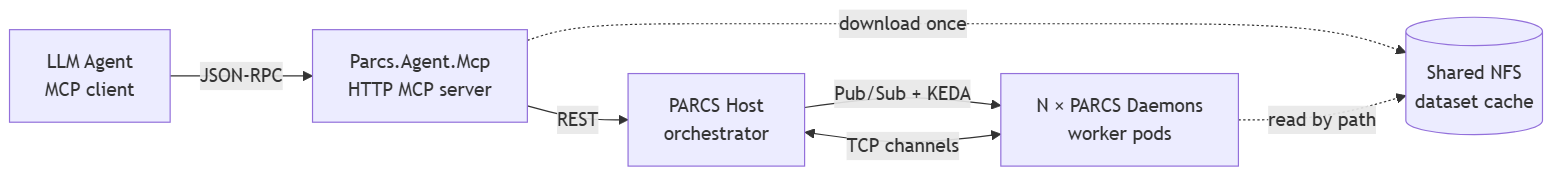
\includegraphics[width=0.85\linewidth]{figures/fig1-architecture}%
}{%
    \fbox{\parbox[c][6em][c]{0.85\linewidth}{\centering\footnotesize\itshape
        [Fig.~1 placeholder --- render \texttt{figures/fig1-architecture.mmd}
        to PNG/PDF and place at \texttt{figures/fig1-architecture.png}]}}%
}
\end{center}
\citfigcaption{1}{%
    \foreignlanguage{ukrainian}{Виконавчий потік PARCS-Agent: агент взаємодіє з MCP-сервером у Kubernetes, який компілює подану логіку, диспетчеризує її через PARCS Host і повертає результати.}%
}{%
    PARCS-Agent execution flow: the agent communicates with a Kubernetes-resident MCP server, which compiles agent-supplied code, dispatches it through the PARCS Host, and propagates results back. KEDA scales daemon pods on demand; bulk inputs traverse a shared NFS volume rather than the protocol.%
}

The architecture has two characteristic properties worth highlighting. First, all parallelism is encapsulated below the MCP boundary, so that the agent only observes synchronous tool invocations. Second, bulk input data does not transit the protocol: the MCP server retrieves a referenced URL once into a shared volume and provides each worker with an identical on-disk path, eliminating per-worker file replication that would otherwise occur.

\medskip\noindent\textbf{The MCP tool surface}\par\nopagebreak
The MCP server exposes four tools, summarised in Table~1. The tool definitions correspond directly to the production source \texttt{ParcsAgentTools.cs} in~\cite{bohusevych2026parcs}.

\cittabcaption{1}{%
    \foreignlanguage{ukrainian}{Інструменти MCP-сервера PARCS-Agent.}%
}{%
    PARCS-Agent MCP tool surface.%
}
\begin{center}
\small
\begin{tabularx}{\dimexpr\linewidth-1cm\relax}{|>{\raggedright\arraybackslash}p{2.6cm}|>{\raggedright\arraybackslash}X|>{\raggedright\arraybackslash}X|>{\raggedright\arraybackslash}X|}
\hline
\textbf{Tool} & \textbf{Purpose} & \textbf{Key inputs} & \textbf{Returns} \\
\hline
\texttt{get\_cluster\_info} & Capability discovery & --- & \texttt{\{workerNodeCount, maxParallelism, daemonCpuRequestMillicores\}} \\
\hline
\texttt{create\_session} & Compile and register an \texttt{IAgentComputation} class & \texttt{sourceCode} (C\#) & \texttt{\{sessionId\}} or \texttt{\{error\}} with diagnostics \\
\hline
\texttt{run\_layer} & Execute a layer in parallel; block until completion & \texttt{sessionId, parallelism, previousLayerId?, customData?, parameters?, datasetUrl?} & \texttt{\{layerId, status, totalElapsedSeconds, successCount, failureCount, result\}} \\
\hline
\texttt{list\_sessions} & Enumerate active sessions & --- & \texttt{[\{sessionId, createdAt, \dots\}]} \\
\hline
\end{tabularx}
\end{center}

The surface is deliberately minimal. There is no fire-and-forget execution variant of \texttt{run\_layer}, no explicit polling endpoint, and no client-side reduction primitive; each such addition would introduce concepts to the agent's prompt without enlarging the class of computations the agent is able to express. Three properties of the design merit explicit discussion.

\textit{Verbose tool descriptions as prompt content.}\quad Each tool's \texttt{[Description]} attribute provides explicit parameter bounds, example values, and the expected response contract. This design responds to the finding~\cite{luo2025mcpsmelly} that the majority of public MCP tools insufficiently document their parameters. The descriptions are concise enough to fit within typical LLM context windows, yet detailed enough to reduce the incidence of malformed agent calls.

\textit{Reference-based result passing.}\quad The \texttt{run\_layer} tool returns a \texttt{layerId}; subsequent layers reference prior outputs through \texttt{previousLayerId} rather than re-transmitting the full result payload. The MCP server retrieves the stored result internally and exposes it to each worker through \texttt{input.PreviousLayerResultJson}. Hence, potentially large JSON payloads are not sent through the LLM context twice --- once on the way out and once on the way back in. The response payload, in turn, returns \texttt{result} as a structured nested object rather than an escaped JSON string, eliminating Unicode-escaped quotes from string-in-string payloads and further reducing token consumption.

\textit{Failure semantics that preserve session state.}\quad A compilation error is reported as \texttt{\{error\}} from \texttt{create\_session} without affecting earlier sessions. A worker exception during \texttt{run\_layer} is reported with \texttt{status: "Failed"} and accompanying diagnostic detail, including a hint when the failure mode is recognisable (e.g. out-of-memory). The session itself remains usable; recovery proceeds by submitting corrected source through \texttt{create\_session} and resuming with the last successful \texttt{layerId} passed as \texttt{previousLayerId}. No prior work is lost. This semantics accommodates the observation that LLMs occasionally produce correct code only on a second attempt, in which case a less forgiving protocol would force redundant re-execution of already-completed work.

\medskip\noindent\textbf{The layer execution model}\par\nopagebreak
A computation is decomposed into a sequence of \emph{layers}. Each layer comprises a parallel fan-out across $N$ workers, a barrier, and a single aggregated JSON value that constitutes the input to the subsequent layer. This fan-out~/~barrier construct is the only execution primitive exposed to the agent; the protocol provides no direct support for point-to-point communication, scatter--gather, or shared memory.

The agent-side contract is the single-method interface \texttt{IAgentComputation} from \texttt{Parcs.Agent.Runtime}:

\begin{lstlisting}
public interface IAgentComputation
{
    Task<AgentLayerResult> ExecuteAsync(
        AgentLayerInput input, CancellationToken ct = default);
}
\end{lstlisting}

The \texttt{AgentLayerInput} type exposes the fields \texttt{WorkerIndex}, \texttt{TotalWorkers}, \texttt{PreviousLayerResultJson}, \texttt{CustomData}, \texttt{Parameters}, and \texttt{DatasetPath}; the worker returns either \texttt{AgentLayerResult.Ok(outputJson)} or \texttt{AgentLayerResult.Error(message)}. The body of \texttt{ExecuteAsync} is written by the agent as straight-line C\#, in the same paradigm as within a single-threaded sandbox. Fan-out, fan-in, JSON marshalling, and inter-worker isolation are the responsibility of the platform.

\begin{center}
\IfFileExists{figures/fig2-sequence.png}{%
    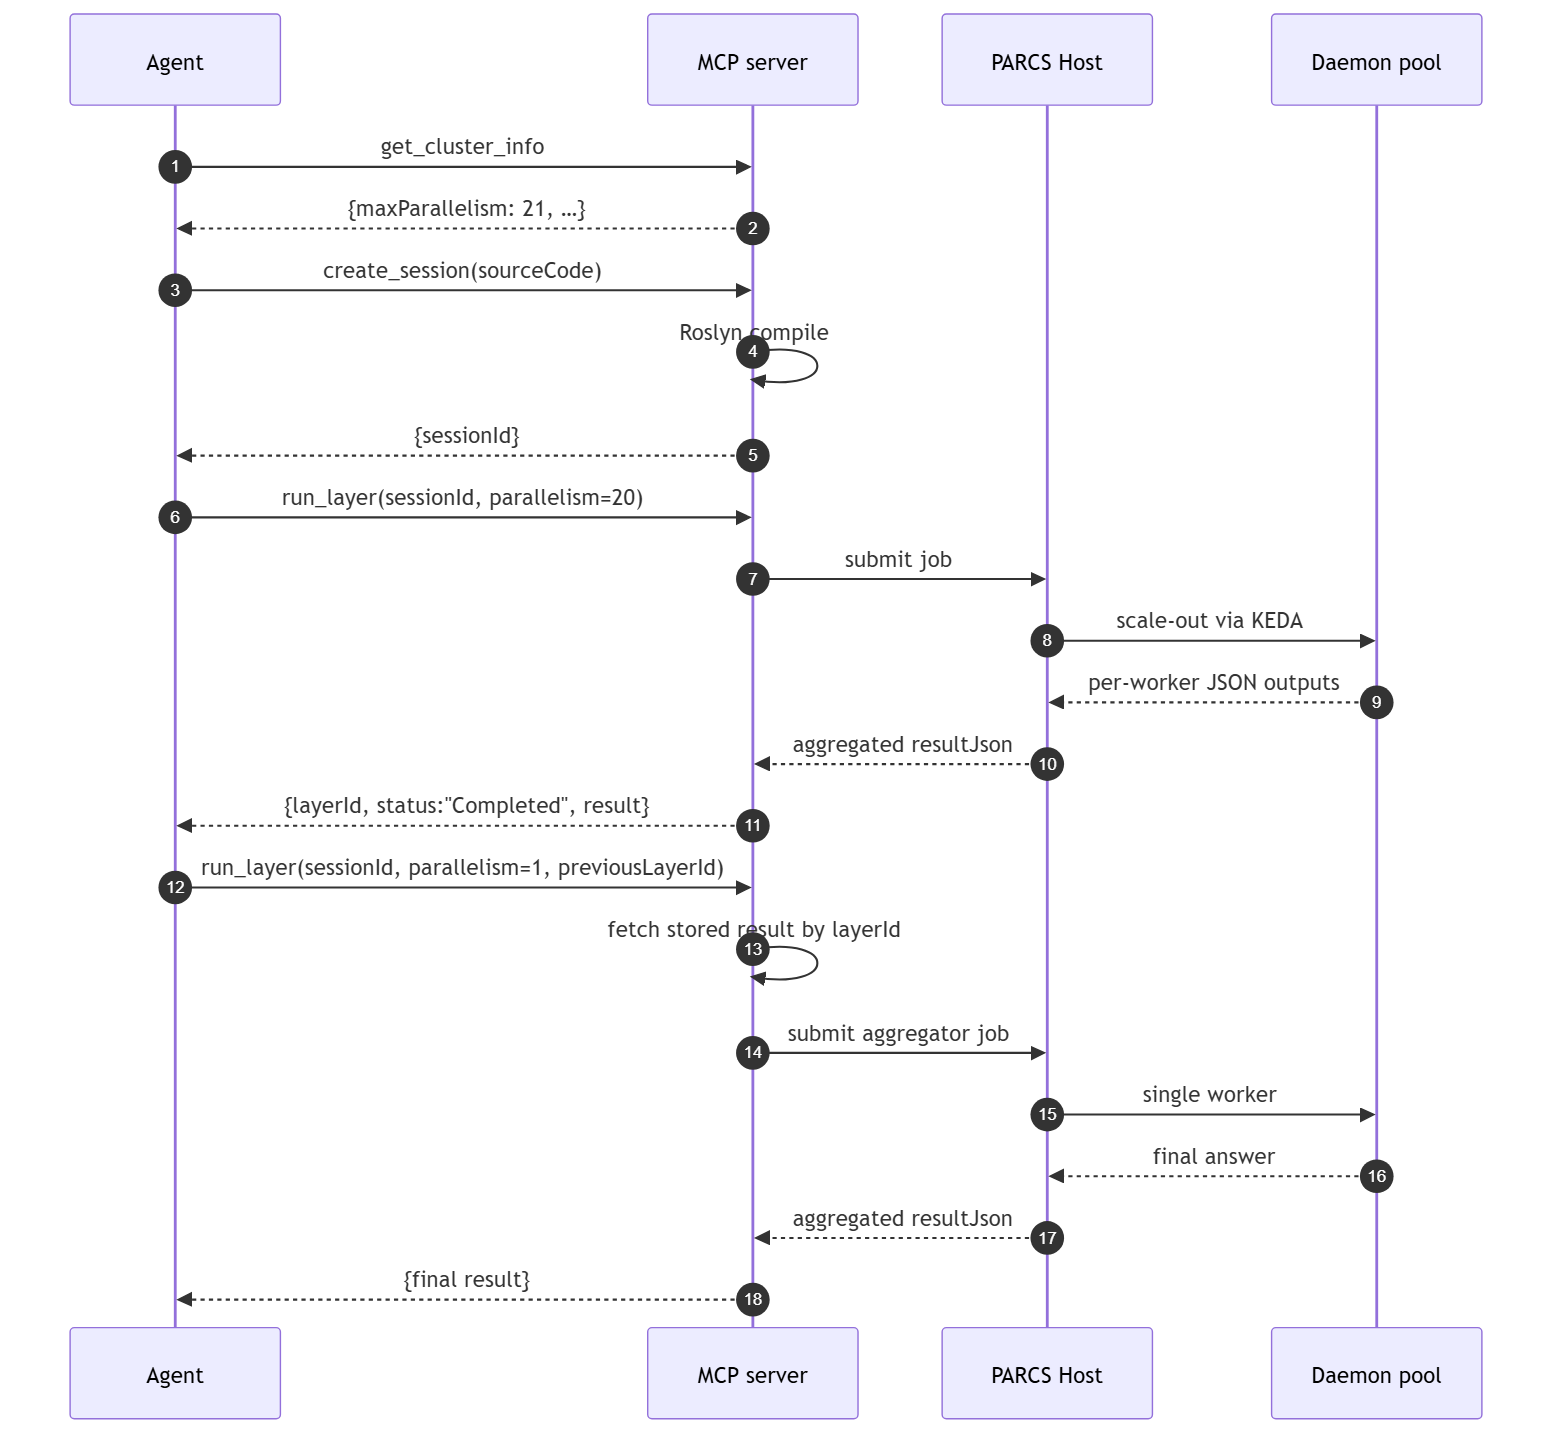
\includegraphics[width=0.85\linewidth]{figures/fig2-sequence}%
}{%
    \fbox{\parbox[c][6em][c]{0.85\linewidth}{\centering\footnotesize\itshape
        [Fig.~2 placeholder --- render \texttt{figures/fig2-sequence.mmd}
        to PNG/PDF and place at \texttt{figures/fig2-sequence.png}]}}%
}
\end{center}
\citfigcaption{2}{%
    \foreignlanguage{ukrainian}{Послідовність двошарового агентного обчислення: виявлення можливостей виконується одноразово; \texttt{create\_session} компілює код агента; \texttt{run\_layer} викликається один раз на шар.}%
}{%
    Sequence of a representative two-layer agent computation. Capability discovery is performed once; \texttt{create\_session} compiles the agent's code; \texttt{run\_layer} is invoked once per layer, with the prior layer's output threaded forward by reference.%
}

\textit{Dataset distribution.}\quad Many agent workloads consume a large shared input such as a covariance matrix, a feature table, or a corpus file. Marshalling such inputs through the protocol replicates the data across workers and burdens the MCP transport. To address this, \texttt{run\_layer} accepts an optional \texttt{datasetUrl} argument. The MCP server downloads the referenced resource once into a content-addressed directory on a shared NFS volume mounted by all daemons at the same path, and exposes that path to each worker via \texttt{input.DatasetPath}. Subsequent layers referencing the identical URL retrieve the file from the local cache without further transfer. The mechanism is transport-agnostic and supports any HTTP-reachable source, including HuggingFace, Google Cloud Storage, Azure Blob Storage, and private object stores.

\textit{Choice of execution language.}\quad PARCS is implemented in .NET, existing modules are distributed as .NET assemblies, and Roslyn provides a JIT-quality compiler accessible from the same process as the MCP server. Using C\# preserves a single compilation and execution stack from agent input to worker output. The choice carries a trade-off: the agent must produce C\# rather than Python, the language more frequently encountered in LLM pre-training data. In practice, frontier models handle the language without measurable quality degradation, in part because the generated code consists of straight-line procedural logic and contains no platform-specific parallel constructs.

\medskip\noindent\textbf{Case study: Monte Carlo Value-at-Risk}\par\nopagebreak
The case considered in this subsection is drawn from a benchmark harness developed alongside the system but reserved for a future evaluation publication. The task is canonical in quantitative finance: estimation of the 1-day 99\,\% Value-at-Risk (VaR) and Conditional Value-at-Risk (CVaR) of a portfolio of 50 equally weighted assets whose return covariance matrix $\Sigma$ is generated from a fixed random seed. The reference protocol specifies $200\,000$ Monte Carlo scenarios distributed across 20 workers at $10\,000$ scenarios each --- a sample count for which a single-threaded sandbox is poorly suited and which is naturally addressed by fan-out across the cluster's worker pool.

The decomposition produced by the agent, following the system-prompt scaffold provided to it, comprises two layers preceded by a capability-discovery call:

\begin{enumerate}[leftmargin=1.5cm,topsep=2pt,itemsep=2pt]
  \item \textbf{Capability discovery.} A single invocation of \texttt{get\_cluster\_info} returns \texttt{maxParallelism}, the upper bound used to size subsequent layers.
  \item \textbf{Layer 1 --- parallel sampling (\texttt{parallelism = 20}).} Each worker draws $10\,000$ Gaussian scenarios using \texttt{new Random(WorkerIndex * 1000 + 42)} together with the shared Cholesky factor of $\Sigma$, computes the per-scenario portfolio loss, and returns its loss vector serialised as JSON.
  \item \textbf{Layer 2 --- aggregation (\texttt{parallelism = 1}).} A second invocation of \texttt{run\_layer} is issued with \texttt{previousLayerId} set to the identifier of layer~1; the server retrieves the stored result, and the single worker reads it from \texttt{input.PreviousLayerResultJson}. The worker concatenates the loss vectors into the full sample of $200\,000$ losses, computes the empirical 99th percentile (the VaR estimate) and the conditional mean above it (the CVaR estimate), and returns \texttt{\{var\_99, cvar\_99\}}.
\end{enumerate}

A representative excerpt of the worker layer is shown below:

\begin{center}
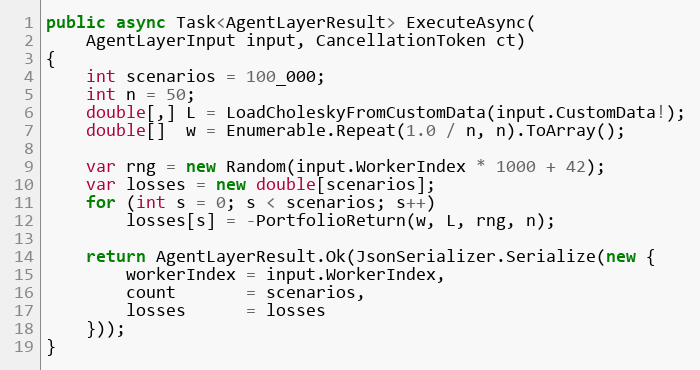
\includegraphics[width=0.85\linewidth]{sources/source1.cs.png}
\end{center}

The implementation contains no synchronisation primitives, no channel construction, and no thread-pool configuration. The worker is functionally equivalent to a single-threaded estimator parameterised by a different random seed. Deterministic per-worker seeding from \texttt{WorkerIndex} ensures disjoint random streams. The output is plain JSON because \texttt{outputData} is a string-typed field at the platform interface.

The case study illustrates four architectural properties of the system.

\begin{enumerate}[leftmargin=1.5cm,topsep=2pt,itemsep=2pt]
  \item \textit{The agent provides only per-worker logic.} Fan-out across 20 workers, the barrier between layers, and the propagation of layer~1's output to layer~2 via \texttt{previousLayerId} are all platform concerns invisible to the agent.
  \item \textit{Aggregation reuses the parallel primitive.} The reducer in layer~2 is a \texttt{run\_layer} invocation with \texttt{parallelism = 1}. The protocol does not distinguish a ``map'' phase from a ``reduce'' phase; \texttt{parallelism} is a numeric parameter rather than a semantic mode.
  \item \textit{Recoverable failure preserves session state.} If the first compilation attempt is rejected --- a realistic occurrence given the difficulty LLMs encounter with C\# numeric generics --- the agent invokes \texttt{create\_session} again with corrected source. The artefacts of the failed compilation are discarded; layer~1 has not yet been executed and no prior work is lost. Should the failure occur during layer~2 instead, the agent retries \texttt{run\_layer} with the same \texttt{previousLayerId}, referencing the still-stored layer~1 result and avoiding re-execution of the sampling step.
  \item \textit{Dataset distribution decouples from worker count.} In an extension where $\Sigma$ is loaded from a multi-megabyte file rather than transmitted as \texttt{customData}, the agent provides a \texttt{datasetUrl} argument on the first \texttt{run\_layer} call. Subsequent layers referencing the same URL incur no additional transport cost regardless of the number of workers.
\end{enumerate}

The case study is not a benchmark and asserts no claim about wall-clock duration or solution quality. Its purpose is to ground the architectural description in concrete agent behaviour and to demonstrate that the synchronous coding paradigm is preserved end-to-end while parallel execution is delivered transparently beneath it.

% sections/04-conclusion.tex --- Висновки та перспективи подальшого дослідження.

\citsection{Conclusions and further research}

This paper presented PARCS-Agent, an architectural pattern in which a Model Context Protocol server provides the interface between a language-model agent and a Kubernetes-based PARCS distributed computing cluster. The contribution is positioned at three complementary levels. At the architectural level, a session--layer--worker hierarchy decouples the agent's reasoning steps from cluster orchestration. At the protocol level, four MCP tools --- capability discovery, session compilation, blocking layer execution, and session enumeration --- align with the agent's step-wise decomposition without imposing distributed-computing concepts on the agent's prompt. At the methodological level, runtime compilation of agent-supplied per-worker logic preserves the synchronous coding paradigm at the agent's surface while delivering parallel execution beneath it, thus circumventing the documented difficulty LLMs encounter when generating parallel code directly.

Three design decisions from this work are worth conserving within similar systems. First, the treatment of MCP tool descriptions as load-bearing prompt content reduces the rate of malformed agent calls. Second, the addressing of layer results by identifier rather than by value --- wherein the agent references prior outputs through \texttt{previousLayerId} while the server retrieves the stored payload internally --- bounds the agent's reasoning trace independently of result size and removes a class of state-management concerns from the protocol surface. Third, the distribution of bulk inputs through a content-addressed shared-storage side channel bounds the protocol payload independently of dataset volume and worker count.

Several directions remain open for further investigation. The most immediate is \textit{quantitative evaluation}: a benchmark of compute-bound agent tasks measuring wall-clock duration, solution quality, token consumption, and operational cost relative to a single-threaded sandbox baseline. A companion harness has been developed for this purpose and is reserved for a separate publication. \textit{Multi-language \texttt{IAgentComputation} support} (Python, F\#) would lower the entry barrier for agents whose pre-training distribution emphasises languages other than C\#. A \textit{GPU-backed daemon pool} would extend the architectural pattern to neural-network training and inference workloads. A \textit{cost-aware scheduling} component would enable cloud deployments to balance throughput and operational expenditure without involving the agent in operational concerns. A \textit{formal security model} would be required to address the multi-tenant trust boundary characteristic of any production deployment. The protocol itself appears stable; future development is anticipated to extend the runtime rather than to modify the agent-facing interface.


% ---- References
\citrefheading{References}
\renewcommand{\refname}{}
% unsrt orders by citation order to keep numbering aligned with the
% hand-numbered Ukrainian list in bib/bibliography-uk.tex.
\bibliographystyle{unsrt}
\bibliography{bib/references}

\end{document}
